\documentclass[main.tex]{subfiles}
\usepackage{tikz}
\usetikzlibrary{positioning,calc}
\usepackage{pgfplots}

\begin{document}
\section*{ASTR 100/1 Lab 3: Angular Size vs. Distance}
In groups at each table, you will investigate how the angular diameter of a spherical body (a ball) depends on its distance from you.

\subsection*{1. Data and Graph}
\begin{enumerate}
\item At your table, discuss and agree on a plan for how to make measurements of the sphere to explore the relationship between its angular size and distance. Consider:
	\begin{enumerate}[a.]
	\item What distances will you make measurements from?
	\item How will you measure the distances?
	\item Will you repeat the measurement with different people? (This is called replication.)
	\item What will you do if points disagree?
	\end{enumerate}

\item Make sure each person makes \textbf{at least one} measurement of the ball's angular size and distance. Record your measurement below.
	\begin{enumerate}
	\item Angular diameter of ball (to nearest half-degree): \rule{2cm}{.15mm}
	\item Distance from ball: \rule{2cm}{.15mm}
	\end{enumerate}
    
\textbf{Record all your measurements on the table worksheet}. Mark the the position of your measurements at your table to \textbf{graph all the points in the table worksheet.}

\item Select someone at your table to \textbf{graph all the points in the table worksheet.}
\end{enumerate}

\subsection*{2. Interpreting the Graph}
Look over the points plotted by your group and discuss the following:
\begin{enumerate}
\item Do the points exhibit a pattern? How would you describe that pattern in words?
\item How might you describe the relationship mathematically?
\item Do all the points agree with each other? What factors might explain the differences we see?
\end{enumerate}

\subsection*{3. Angular Size of Astronomical Objects}
\begin{enumerate}
\item Let's consider the Sun.
	\begin{enumerate}[a.]
	\item Does the Sun's angular size changes during the year?
	\item What month is it the smallest? \rule{2cm}{.15mm}
	\end{enumerate}

\item Now let's look at the Moon.
	\begin{enumerate}[a.]
	\item Is the Moon larger when it's full?
	\item What is a supermoon?
	\item Is the Moon larger when it's near the horizon?
	\end{enumerate}

\end{enumerate}

The planet Mars shows the greatest variation in size of all the planets, which we will explore here.
\begin{enumerate}
\item In groups of 2-3, start up Stellarium. Find where Mars is today. You can turn off the atmosphere (hit A) and ground (hit G) to help. 
\item Once you have found Mars, you can click on it and center the view (by pressing the space key). Take note of Mars's angular diameter (given as ``Apparent diameter" in the left-hand side info panel.
\item Zoom in until Stellarium renders some surface features.
\item You are going to look at how Mars's \textbf{angular diameter} and \textbf{right ascension (``RA")} values each change over time. To do this, open the Date/Time window and vary the date from October 2021 to October 2023, one month at a time. At each date, take note of Mars's \textbf{angular diameter} and \textbf{right ascension (``RA")}. These are the values you will plot (\textbf{NOT} the date!).
\item Plot Mars's angular diameter vs. right ascension in the grid below and answer the following questions.
\begin{figure}[htb]
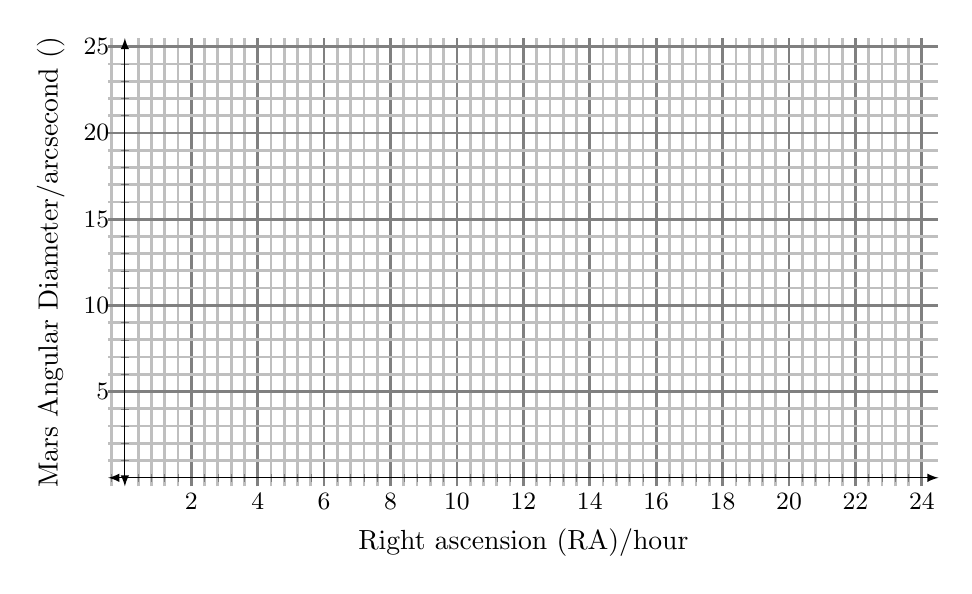
\begin{tikzpicture}
\begin{axis}[
	width=\textwidth,
    height=0.6\textwidth,
    xmin=0,xmax=24,
    ymin=0,ymax=25,
    grid=both,
    grid style={line width=1pt, draw=gray!50},
    major grid style={line width=1pt, draw=gray!100},
    axis lines=center,
    minor tick num=4,
    enlargelimits={abs=0.5},
    axis line style={latex-latex},
    ticklabel style={font=\small},
    xlabel near ticks,
    ylabel near ticks,
    xlabel={Right ascension (RA)/hour},
    ylabel={Mars Angular Diameter/arcsecond (\si{\arcsecond})}
]
\end{axis}
\end{tikzpicture}
\end{figure}

	\begin{enumerate} [a.]
    \item How big is Mars in October 2021? \rule{2cm}{.15mm} arcseconds
    \item Where is it in its orbit in October 2021?
    \item In what month is Mars largest? \rule{2cm}{.15mm} 
    \item How big is it that month? \rule{2cm}{.15mm}  arcseconds
    \item What explains the pattern of sizes you find in your graph?
	\end{enumerate}

\end{enumerate}

\subsection*{4. Lab Quiz on Moodle}
Go to the Lab 3 section on the Moodle page and complete the End-of-Lab Quiz. Write your name on the Table Worksheet and hand it in.


%\textbf{For Sunset Project}: The goal for the project is to get a second photo at least 1 week after the first and a third photo at least 4 weeks after the first (and at least 1 week after the second), all from the same location. If you haven't gotten a successful first photo yet. Get one soon or you will run out of time. If you did get a successful first photo and uploaded it by the original due date, a bonus point for you!

\end{document}